\setcounter{rownumber}{0}
\chapter{A Coherently Stimulated Phonon Spectrometer}
\label{ch:CoBS}
\acresetall

\hfill

\textit{This chapter presents a preview of an article in-prep for publication. Neither the author nor the publisher are responsible for any errors or omissions in any future publication derived from this version of the manuscript.}

\doublespacing

\section{Abstract}
We present a novel coherently stimulated Brillouin spectrometer utilizing a detuned pump-probe design that exploits a relaxation of phase-matching requirements at small lengths, enabling room-temperature traveling-wave phonon spectroscopy at the micrometer scale with sub-\SI{10}{\femto\watt} sensitivity. This approach overcomes the limitations of traditional stimulated Brillouin techniques, particularly regarding phase-matching constraints and spatial resolution. We validated our instrument’s sensitivity with \SI{1}{\centi\meter} of \ac{UHNA3} fiber and \SI{100}{\micro\meter} of bulk carbon disulfide liquid, demonstrating its capability to measure Brillouin scattering in materials with low Brillouin gain or, with particular advantage, small effective lengths. This advancement opens new possibilities for nanometer-scale Brillouin spectroscopy and the development of nano-acousto-optic devices.

\section{Introduction}
\label{sec:Introduction}

Brillouin scattering, the inelastic interaction between light and acoustic phonons, is a fundamental phenomenon for probing the mechanical and structural properties of materials at microscopic scales. In spontaneous Brillouin scattering, thermally excited acoustic phonons scatter incident light, causing frequency shifts that reveal information about the material’s elastic properties and acoustic modes \cite{boyd2020nonlinear}. However, the weak signal inherent to spontaneous Brillouin scattering often demands long acquisition times and limits spatial resolution, posing challenges for high‐resolution material characterization.

\ac{SBS} uses intense optical fields to amplify the acoustic wave through a nonlinear optical process \cite{chiao1964stimulated}. In \ac{SBS}, a strong pump laser interacts with a counter‐propagating Stokes wave in the medium, generating acoustic phonons via electrostriction. As the phonon population grows, it further amplifies the Stokes wave. In turn, that amplified Stokes wave interferes with the pump and reinforces the acoustic field, creating a positive feedback loop that drives exponential amplification. This mechanism enables more efficient excitation and detection of acoustic phonons and underpins numerous applications in optical signal processing, sensing, and high‐resolution spectroscopy including mechanobiology \cite{eggleton2013inducing, fotiadi2023brillouin, kobyakov2009stimulated, ippen1972stimulated, speziale2014brillouin, palombo2019brillouin, dil1982brillouin, eggleton2019brillouin, prevedel2019brillouin, conrad2019mechanical}.

%this whole paragraph needs to be rewritten to set up the phase matching restricitons that continue to pose a challenge\cite{yu2024chip} as a thing that my method solves.
However, conventional \ac{SBS} techniques struggle with short samples or materials of inherently low Brillouin gain and strict phase matching requirements continue to pose a challenge. \cite{rakich2012giant, gyger2020observation, yu2024chip}. Because the Stokes amplitude depends on the product of the Brillouin gain coefficient, pump power, and interaction length, small volumes often yield weak signals unless extremely high optical powers are used. Moreover, while backward \ac{SBS} sends the scattered wave in the opposite direction of the pump, parasitic reflections and pump leakage can still obscure the Stokes signal, demanding careful optical isolation and sometimes elaborate filtering. These constraints make it difficult to measure thin films and micro‐ and nanoscale devices, particularly if high optical intensities risk damaging sensitive samples. As a result, standard \ac{SBS} approaches are not easily adapted to sub‐centimeter lengths or low‐gain media, prompting the need for new methods that maintain high sensitivity in short interaction regions.

To overcome these challenges, researchers have explored various approaches \cite{shin2013tailorable, van2015interaction, kittlaus2016large, djadaojee2020stimulated, gusev2018advances, gerakis2011coherent}. Techniques based on optical cavities increase the effective interaction length, but require precise alignment and are sensitive to environmental fluctuations \cite{pant2011cavity}. Forward Brillouin scattering methods, such as those demonstrated by Kittlaus et al. \cite{kittlaus2017chip}, offer relaxed phase‐matching conditions but introduce increased modal complexity. Meanwhile, coherent probe beam amplification can boost sensitivity, yet it can introduce additional noise and complexity because phase noise in laser sources can cause significant gain fluctuations \cite{shlomovits2015effect}.

Here, wedemonstrate a detuned pump–probe design that relaxes the usual phase‐matching constraints at short lengths. This approach offers a new route to measure traveling‐wave phonons in sub‐centimeter or even micrometer‐scale samples at room temperature with unprecedented sensitivity. We demonstrate the capabilities of the instrument by measuring Brillouin scattering in \SI{1}{\centi\meter} of \ac{UHNA3} fiber and \SI{100}{\micro\meter} of bulk carbon disulfide (\ce{CS2}) liquid. These measurements highlight the instrument’s ability to characterize materials with low Brillouin gain or small effective lengths.

The development of this coherently stimulated Brillouin spectrometer opens new avenues for nanometer‐scale Brillouin spectroscopy and advances the characterization and design of nano‐acousto‐optic devices. It holds promise for pushing research in material science, photonics, and sensing technologies toward higher spatial resolution and sensitivity, marking a significant step toward practical, room‐temperature Brillouin‐based spectroscopy and sensing solutions.

\section{Theoretical Framework}
\label{Theoretical Framework}

\subsection{Coherently Stimulated Four-Wave Brillouin Scattering}
\label{Theoretical Framework:Coherently stimulated five-wave Brillouin scattering}

\begin{figure}[t]
    \centering
    \begin{subfigure}[b]{0.37\textwidth}
        \centering
        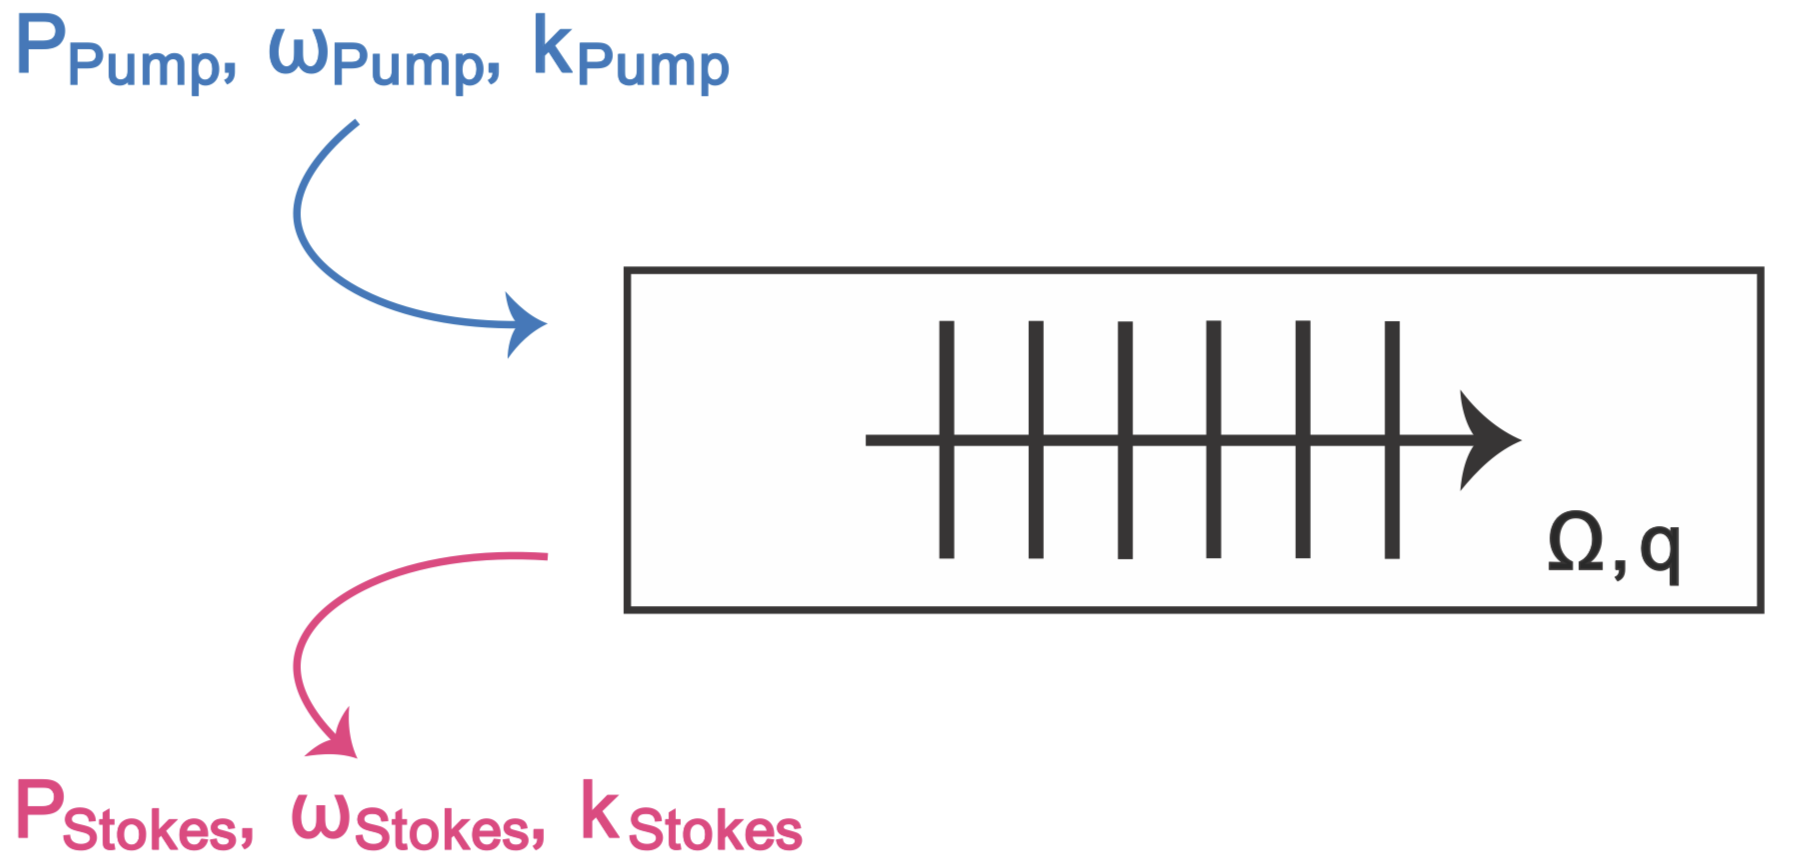
\includegraphics[width=\textwidth]{figs/3-CoBS/SBS Illustrator Diagram.png}
        \caption{}
        \label{fig:CoBS:SBSDiagram}
    \end{subfigure}
    \hfill
    \begin{subfigure}[b]{0.54\textwidth}
        \centering
        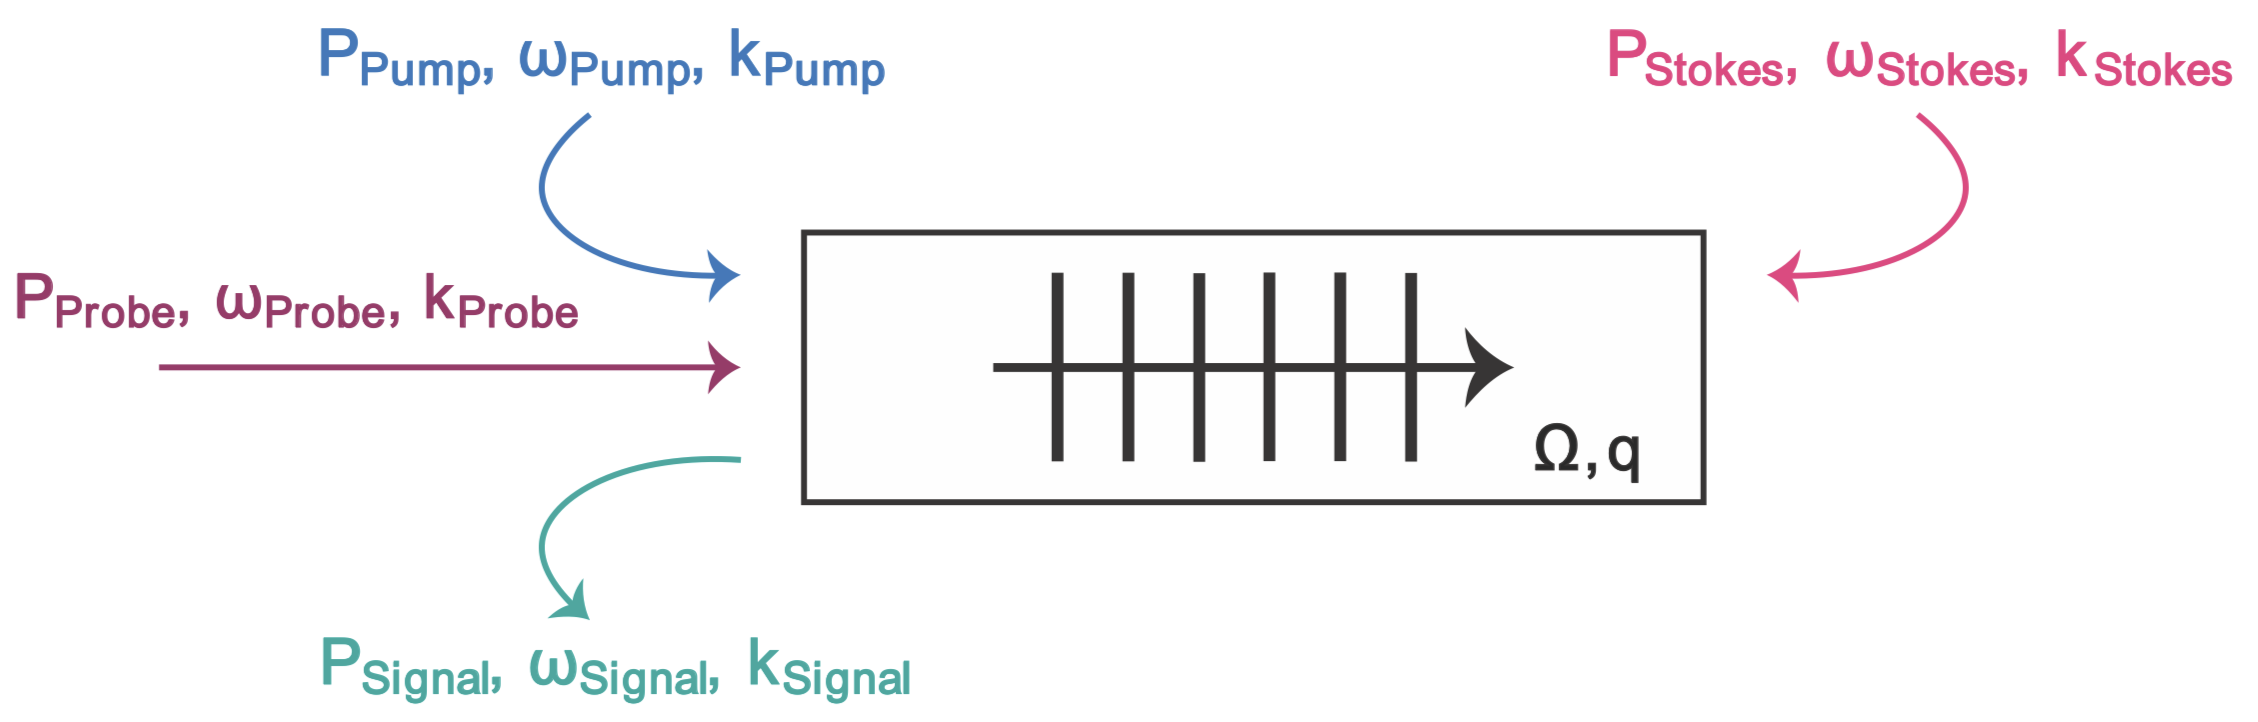
\includegraphics[width=\textwidth]{figs/3-CoBS/4-Wave-Brillouin-Scattering.png}
        \caption{}
        \label{fig:CoBS:4-Wave-Brillouin-Scattering}
    \end{subfigure}
    \caption{Figure~\ref{fig:CoBS:SBSDiagram} illustrates standard (three‐wave) stimulated Brillouin scattering (\acs{SBS}), showing a single optical pump field \(P_{\mathrm{Pump}}\), the backscattered Stokes field \(P_{\mathrm{Stokes}}\), and the acoustic (phonon) wave of frequency \(\Omega\) and wavevector \(q\). Here, \(\omega_{\mathrm{i}}\) and \(k_{\mathrm{i}}\) represent the frequency and wavevector of the optical fields, respectively. Figure~\ref{fig:CoBS:4-Wave-Brillouin-Scattering} illustrates coherently stimulated (four‐wave) Brillouin scattering (\acs{CoBS}), where an additional optical probe \(P_{\mathrm{Probe}}\) mixes with the pump to generate both the Stokes wave and a new signal \(P_{\mathrm{Signal}}\), mediated by the same acoustic wave. We refer to this as four‐wave because four optical fields (pump, probe, Stokes, signal) participate, although one may also count the acoustic wave as a “fifth” wave.}
    \label{fig:CoBS:SBSvsCoBSDiagrams}
\end{figure}

Traditional \ac{SBS}, illustrated in Figure~\ref{fig:CoBS:SBSDiagram}, is a three-wave mixing process in which incident pump laser light of frequency \(\omega_{\mathrm{Pump}}\) inelastically scatters from a traveling-wave phonon of frequency \(\Omega\) to produce light that is frequency-shifted by the phonon frequency. In the Stokes process the phonon is retreating from the incident laser light and the scattered light is shifted down in frequency (\(\omega_{\mathrm{Stokes}} = \omega_{\mathrm{Pump}} - \Omega\)). Spatial overlap of the backscattered light with the incident laser light allows for interference of the two optical fields to produce a frequency at the difference of the two (\(\omega_{\mathrm{Pump}} - \omega_{\mathrm{Stokes}}\)). Since this difference frequency is exactly equal to the frequency of the acoustic field \(\Omega\), the beating of the incident pump light with the backscattered Stokes light produces an electrostrictive reinforcement of the acoustic wave. This driving of the acoustic wave in turn increases the scattering rate of the incident pump light, producing a positive feedback process and an exponential increase of the amplitude of the backscattered Stokes wave.

Figure~\ref{fig:CoBS:4-Wave-Brillouin-Scattering} illustrates coherently stimulated four-wave Brillouin scattering for the Stokes process, mediated by an acoustic wave. We introduce a strong, controlled external Stokes wave of frequency \(\omega_{\mathrm{Stokes}}\) that drives electrostrictive reinforcement of the acoustic field in the medium. The backscattered Stokes light is normally collected in an \ac{SBS} process, but the external Stokes laser overwhelms it. To resolve this, weinject light of a distinct frequency \(\omega_{\mathrm{Probe}}\) from an additional external laser which copropagates with the Pump and backscatters in the medium from the strongly driven acoustic field. This produces backscattered Signal light to be collected (\(\omega_{\mathrm{Signal}} = \omega_{\mathrm{Probe}} - \Omega\)) which is spectrally distinct from the high-powered Stokes laser light.

To describe this interaction and characterize the performance of the instrument, wederive the coupled-wave equations for the four-wave mixing process in Appendix~\ref{Appendix:Coupled-Wave Equations}. These equations describe the relationship between the optical fields and the acoustic field in the material and result in the following expression for the scattered power of the backscattered signal,
\\
\begin{equation}
  P_{Sig} = \frac{1}{4}(G_{B}L)^{2}P_{P}P_{S}P_{Pr}sinc^{2}\left(\frac{\Delta kL}{2}\right),
  \label{Eq:Theoretical Framework:Scattered Power}
\end{equation}
\\
where \(P_P\), \(P_S\), and \(P_Pr\) are the powers of the pump, Stokes, and probe lasers, respectively. \(G_B\) is the effective Brillouin gain, given by
\\
\begin{equation}
  G_{B} = \frac{g_{0}}{A_{eff}}\frac{\left(\frac{\Gamma_{B}}{2}\right)^{2}}{(\Omega - \Omega_{B})^{2} + \left(\frac{\Gamma_{B}}{2}\right)^{2}},
  \label{Eq:Effective Brillouin Gain}
\end{equation}
\\
with the on-resonance gain factor of the material given by
\\
\begin{equation}
  g_{0} = \frac{\gamma_{e}^{2}\omega^{2}}{nvc^{3}\rho_{0}\Gamma_{B}}.
\end{equation}
\\
Here, \(\gamma_e\) is the electrostrictive constant, \(\omega\) is the pump frequency, \(n\) is the refractive index of the material, \(v\) is the sound speed of the material, \(c\) is the speed of light, \(\rho_0\) is the mean density of the material, and \(\Gamma_B\) is the Brillouin linewidth, or phonon dissipation rate, of the material. In Equation~\ref{Eq:Effective Brillouin Gain}, \(\Omega_B\) is the resonant Brillouin frequency of the material, \(A_{Eff}\) is the effective area of the material, \(\Delta k\) is the wavevector mismatch between the optical fields, to be discussed next, and \(L\) is the effective length of the material.


\subsection{Phase Matching Relaxation}
\label{Theoretical Framework: Phase matching relaxation}
In all nonlinear optical processes, efficiency is maximized when phase matching conditions are satisfied. A frequency mismatch (energy unconservation) or a wavevector mismatch (momentum unconservation) each result in drastically reduced efficiency of a given process.\cite{maker1962effects} This can be seen by Equation~\ref{Eq:Theoretical Framework:Scattered Power}, where the wavevector mismatch, \(\Delta k\), is contained within a \(\mathrm{sinc^2}\) function. This \(\mathrm{sinc^2}\) term thereby defines the phase matching bandwidth of the system, notably scaling with effective interaction length \(L\).

We apply this wavevector mismatch allowance to the pump and probe waves (\(\Delta k = k_{\mathrm{Pump}} - k_{\mathrm{Probe}}\)) so that the backscattered signal is different than the applied Stokes wave. This choice allows for selection of the signal and rejection of the Stokes with a bandpass filter. Expressed in terms of wavelengths, this gives
\\
\begin{equation}
  \Delta k = \frac{4\pi n\Delta\lambda}{\lambda_{Pump}\lambda_{Probe}} \approx \frac{4\pi n\Delta\lambda}{\lambda_{Pump}^{2}}.
\end{equation}
\\
We can apply this to the phasematching bandwidth term to find the fraction of maximum scattered power, \(\Phi\), that can be expected for a given interaction length, \(L\), and phase mismatch \(\Delta\lambda\) between the pump and probe,
\\
\begin{equation}
  \Phi \equiv sinc^{2}\left(\frac{2\pi n\Delta\lambda L}{\lambda_{Pump}^{2}}\right).
  \label{Eq:Phi}
\end{equation}
\\
Using this expression for \(\Phi\), wesee that for an effective length of \SI{1}{\meter}, a wavelength mismatch of only \SI{0.6}{\pico\meter} from a typical wavelength of \SI{1.55}{\micro\meter} pump light in \ac{UHNA3} fiber drops the scattered power to half of the maximum. However, for shorter effective lengths the wavevector mismatch becomes more forgiving; a \SI{36}{\pico\meter} mismatch preserves 82.5\% of the maximum signal for a length of \SI{1}{\centi\meter} under identical conditions. This separation translates to about \SI{4.5}{\giga\hertz}, providing enough spectral separation for the backscattered signal to be isolated from the applied Stokes light.

Furthermore, for decreasing lengths, Equation~\ref{Eq:Phi} predicts an increase in the fraction of maximum signal produced, given equivalent pump--probe detuning, as the \(\mathrm{sinc^2}\) function is sampled closer to its peak center. Alternatively, as length decreases, the probe may be further detuned from the pump and still achieve the same fraction of the maximum signal as for longer lengths, perhaps offering a slight advantage in noise reduction. It should be noted that the scattered power, as given by Equation~\ref{Eq:Theoretical Framework:Scattered Power}, scales with the square of the effective length. Thus, while smaller lengths allow for the ability to capture a larger fraction of this maximum scattered power, the actual amount of scattered power decreases dramatically as length decreases.

\section{Methods}\label{Methods}
\subsection{Instrument Design}
\label{Methods:Instrument Design}

\begin{figure*}[htbp]
\centering
\vspace{-20mm}
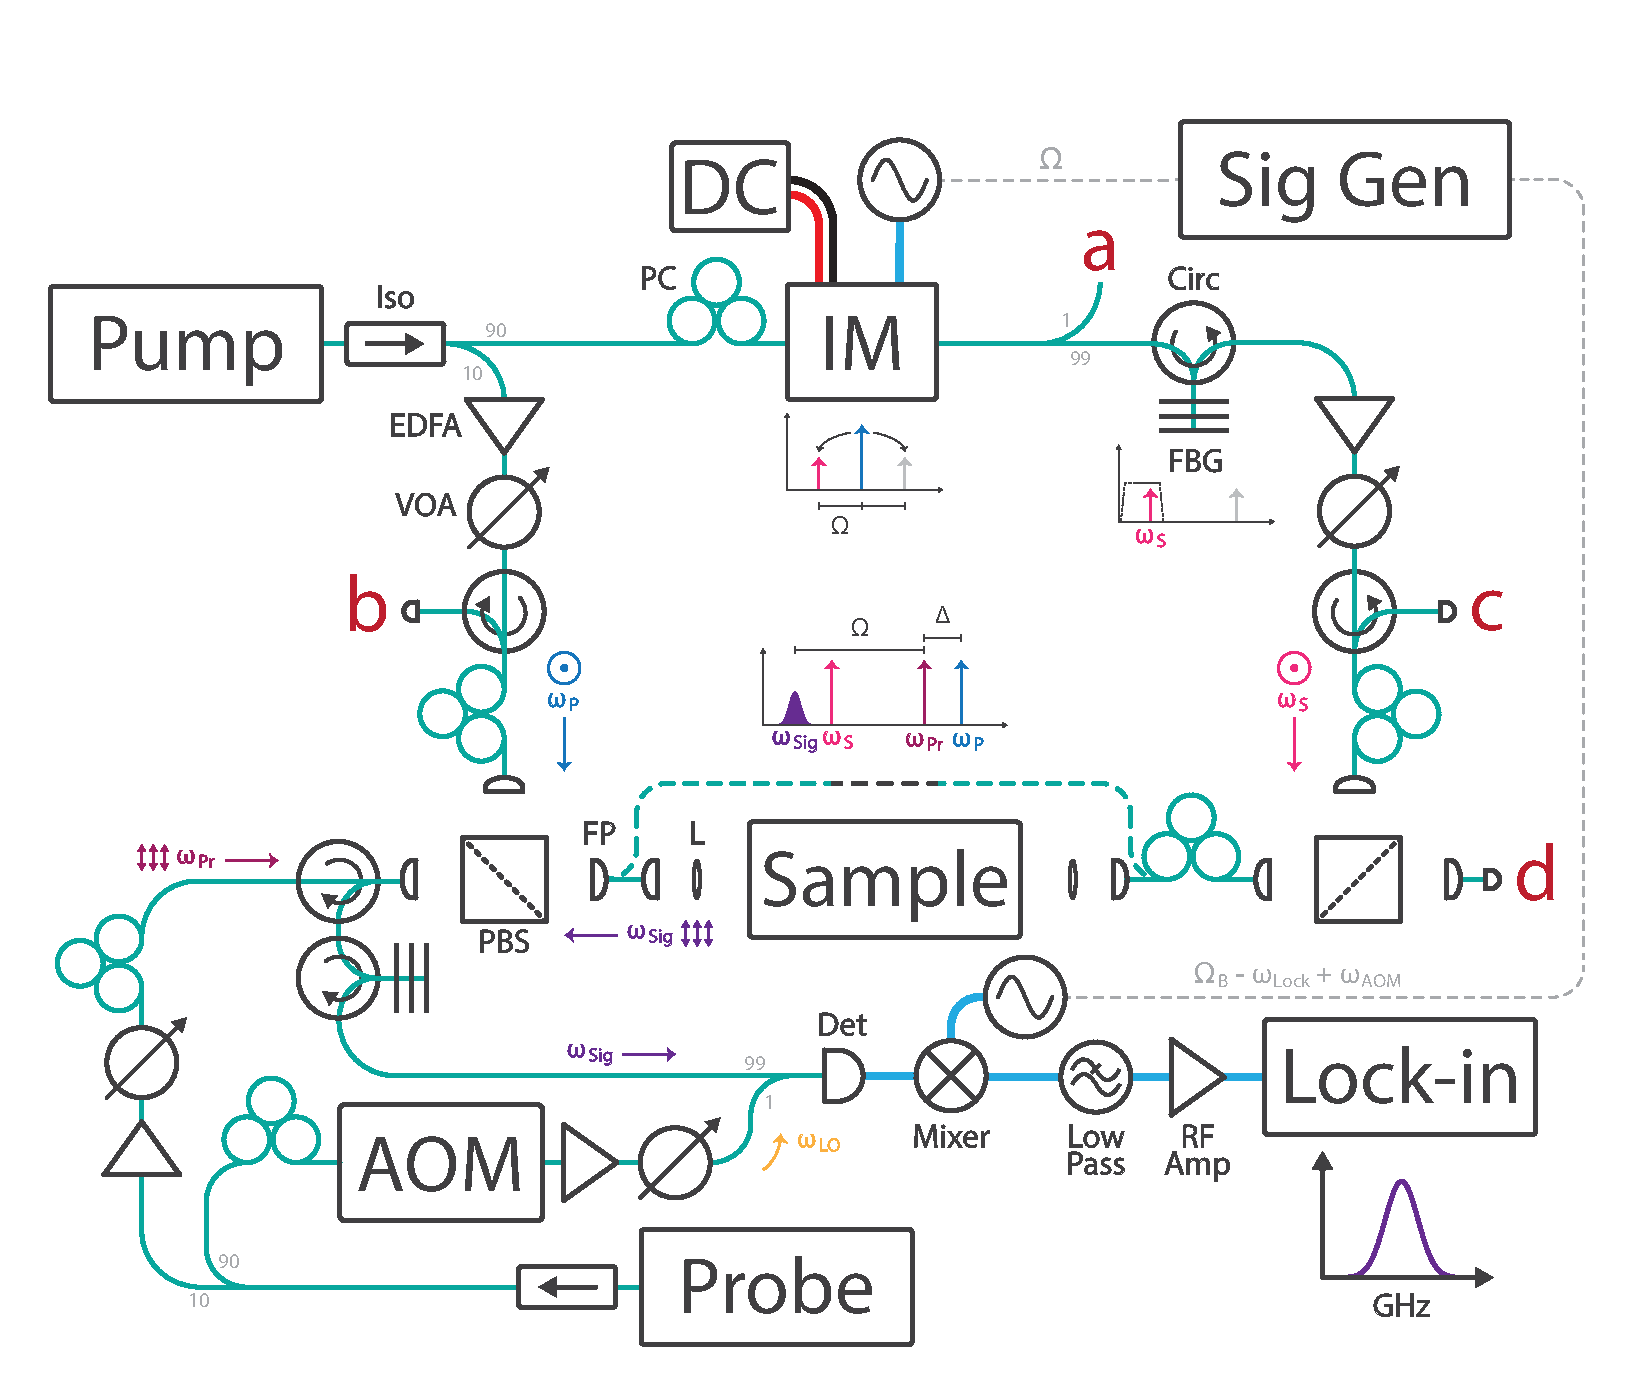
\includegraphics[width=\textwidth]{figs/3-CoBS/Instrument-Design-V1_compat.pdf}
\caption{
Design schematic of a coherently stimulated phonon spectrometer. A tunable \ac{CW} laser at approximately \SI{1.55}{\micro\meter} emits light that passes through an isolator (Iso) and a splitter, diverting 10\% to a \SI{27}{\dBm} \ac{EDFA} followed by a \ac{VOA}. This pump light (\(\omega_P\)) is polarization-controlled to reflect off a \ac{PBS} and is recoupled to fiber via a \ac{FP}, then directed to the sample either by direct fiber coupling or through a pair of \ac{FP}s and lenses (L) for free-space samples. After passing through the sample, the pump light traverses a corrective polarization controller that mitigates fiber twists and bends before reflecting off a second \ac{PBS}, where it is routed to port (c) for power monitoring. To synthesize the Stokes wave, a 90\% split from the original pump is processed through a \ac{IM} and a \ac{FBG}, generating a Stokes sideband downshifted from the pump by \(\Omega\). This frequency shift is swept via a signal generator to capture \(\Omega_B\). A 99/1 splitter provides a tap at port (a) to optimize Stokes synthesis. The Stokes wave (\(\omega_S\)), amplified by a \SI{1}{\watt} \ac{EDFA} and \ac{VOA}-controlled, counter-propagates along the pump path and is monitored at port (b). A second tunable \ac{CW} laser, detuned from the pump, generates the probe wave (\(\omega_{Pr}\)), which is amplified by a \SI{1}{\watt} \ac{EDFA}, attenuated variably, and polarization-controlled to pass through the initial \ac{PBS} where it is incident on the sample. Backscattered signal light (\(\omega_{Sig}\)) transmits back through the \ac{PBS}, while unscattered probe light transmits to a power meter at port (d). A circulator parts the signal from the probe path, with an \ac{FBG} filtering out any unwanted noise or Stokes light. Finally, the signal is heterodyned with an \ac{EDFA}-amplified, \ac{AOM}-shifted \ac{LO} derived from the probe laser and directed to a photodiode for detection. The resulting \ac{RF} signal is mixed with an \ac{AC} \ac{LO} supplied by the signal generator which sweeps synchronously with the Stokes synthesis frequency, and collected by a lock-in amplifier for data processing.
}
\label{fig:Instrument Design}
\end{figure*}

Figure~\ref{fig:Instrument Design} shows the instrument’s design. A pump and Stokes wave is synthesized from a single tunable laser source for coherent stimulation of a sample. The pump wave (\(\omega_{\mathrm{Pump}}\)) is amplified by an \acl{EDFA} and passed through a \acl{VOA} for power control. The output is then polarization-controlled to reflect at a \acl{PBS} for injection into the sample. For Stokes synthesis, an \acl{AC} signal (\(\Omega\)) is supplied to an \acl{IM} with carrier frequency nulled and a tunable filter is used to select the lower-frequency Stokes side band (\(\omega_{\mathrm{Pump}} - \Omega\)). This Stokes light is then amplified by an \ac{EDFA}, passed through a \ac{VOA}, and polarization-controlled to reflect at a second \ac{PBS} for couter-propagation to the pump through the sample.

A separate tunable laser is used to supply a probe wave (\(\omega_{\mathrm{Probe}} = \omega_{\mathrm{Pump}} + \Delta k\)) and \acl{LO}. Probe light is amplified by an \ac{EDFA} and passed through a \ac{VOA} and a polarization controller aligns the polarization for transmission through the first \ac{PBS} whereby it copropagates with the pump through the sample. Backscattered light exits the sample and transmits back through the first \ac{PBS}, whereas the orthogonally polarized Stokes light reflects at this same point to be diverted to a tap for power monitoring. The backscattered signal (\(\omega_{\mathrm{Signal}} = \omega_{\mathrm{Probe}} - \Omega\)) then routes through two subsequent circulators for spectral filtering by a \SI{5}{\giga\hertz} bandpass tunable filter. This filter allows the desired backscattered signal to pass while rejecting any reflected probe light as well as any reflected, transmitted, or backscattered light from the pump or Stokes waves that was not already diverted by the PBS.

The filtered signal then heterodynes via a 99-1 splitter with the \ac{LO} which is frequency-upshifted by an \acl{AOM} (\(\omega_{\mathrm{LO}} = \omega_{\mathrm{Probe}} + \omega_{\mathrm{AOM}}\)) and controlled to be copolarized with the signal. Of the resulting frequencies from the heterodyne process, only the difference frequency term is considered, as all others are beyond the range of detection. This heterodyned signal (\(\omega_{\mathrm{Signal}} = \Omega + \omega_{\mathrm{AOM}}\)) is then captured by a photodiode detector and heterodyned again by a \acl{RF} mixer with a second \ac{AC} signal (\(\Omega + \omega_{\mathrm{AOM}} - \omega_{\mathrm{Lock}}\)), where \(\omega_{\mathrm{Lock}}\) is a fixed-frequency to be detected by a lock-in amplifier set to this frequency after being passed through a low-pass filter and amplified by an \ac{RF} amplifier. Synchronous sweeping of both \ac{AC} signals, each involving \(\Omega\), allows for \(\omega_{\mathrm{Lock}}\) to remain fixed throughout measurement over a frequency range.

\subsection{Experimental Techniques}
\label{Methods:Experimental Techniques}
We optimized the \ac{SNR} of the instrument through specific design choices and device settings. Our setup simultaneously generates pump, Stokes, and probe optical fields for coherently stimulated Brillouin scattering. The pump laser provides \(\sim\!\SI{45}{\milli\watt}\) total output, of which 10\% is split and amplified to \(\sim\!\SI{0.5}{\watt}\) for the pump field; the remaining 90\% is frequency-shifted and amplified to \(\sim\!\SI{1}{\watt}\) for the Stokes field. Likewise, the probe laser also outputs \(\sim\!\SI{45}{\milli\watt}\), with 10\% amplified to \(\sim\!\SI{1}{\watt}\) for the probe field and the remaining 90\% reserved for the \ac{LO}. To combine the backscattered signal and \ac{LO} with minimal loss, weuse a 99/1 splitter instead of a typical 50/50, preserving 99\% of the signal. The \ac{LO} is therefore amplified to \(\sim\!\SI{230}{\milli\watt}\) so the total optical power at the detector remains below the \(\SI{2.4}{\milli\watt}\) damage threshold. After detection, the electronic signal is mixed with a \SI{17}{\dBm} \ac{AC} reference and further amplified by \SI{23}{\dBm} before input to the lock-in amplifier. We find that running both the pump and probe lasers in “whisper” mode (as opposed to “dither”) significantly enhances the measured SNR.

We use a Zurich Instruments HF2LI \SI{50}{\mega\hertz} lock-in amplifier whose demodulator settings are carefully tuned to maximize \ac{SNR}. A \SI{10}{\mega\hertz} reference clock from the signal generator is fed into the lock-in to synchronize timing. The input-signal range, which sets the analog input amplifier’s gain, should exceed the measured signal (including any \ac{DC} offset) by at least a factor of two. This is best achieved by using the lock-in software’s auto feature, which continuously adjusts the range over a rolling \SI{100}{\milli\second} window. We set the input coupling to \ac{AC}, insert a high-pass filter to remove \ac{DC} components, and choose \SI{1}{\mega\ohm} input impedance. For noise suppression, we also engage the lock-in’s eighth-order low-pass filter (roll-off \SI{48}{\decibel\per\octave}) and sample the data at \SI{1.84}{\mega\sample\per\second}, the maximum rate available.

Further \ac{SNR} improvements are gained by narrowing the lock-in’s low-pass filter bandwidth to match both the sub-\si{\hertz} natural linewidth of the heterodyne signal and the thermally-driven frequency drift of the apparatus. After a \(\sim\!\SI{30}{\minute}\) warm-up, we observe less than \SI{100}{\hertz} of drift in the detected signal frequency, so we typically set a \SI{100}{\hertz} low-pass bandwidth for multi-hour measurements. For shorter scans (\(< \SI{15}{\minute}\)), we can reduce this bandwidth to \SI{40}{\hertz} if needed. In addition to linewidth variability, the signal’s center frequency can shift due to thermal changes in the \ac{AOM} and related electronics. Although \(\Omega\) is nominally controlled to sub-hertz precision by the signal generator, our \ac{AOM}’s shift \(\omega_{\mathrm{AOM}}\) drifts from \SI{40}{\mega\hertz} up to \(\sim\!\SI{40.00082}{\mega\hertz}\) over roughly \SI{30}{\minute}. Once at thermal equilibrium, the \ac{AOM} remains stable within \(\pm\SI{50}{\hertz}\), enabling a reliable lock-in frequency reference and minimal filter bandwidth. This stability is crucial for repeatable, high-resolution Brillouin measurements.

\section{Results}\label{Results}
\subsection{Instrument Sensitivity}
\label{Results:Instrument sensitivity}

We begin by testing the sensitivity of the instrument as a way of defining a performance metric for the instrument which can be used to indicate what material, power, and length combinations might be possible to measure. From Equation~\ref{Eq:Theoretical Framework:Scattered Power}, the sensitivity of the instrument is the minimum scattered power, \(P_{Sig}\), to produce a statistically significant measurement. To determine this, we target a specific length, \(L\), of a sample of known effective Brillouin gain, \(G_B\). We keep the pump-probe detuning, \(\Delta\lambda\), constant across measurements and record the pump, Stokes, and probe optical powers to calculate the scattered power. Starting with sufficient optical powers to produce a clearly distinguishable measurement, we gradually reduce the optical powers until the sensitivity floor is reached.

To serve as our sensitivity testbed, we prepared \SI{1}{\centi\meter} of Nufern's \acl{UHNA3} fiber, a well-studied fiber with known effective Brillouin gain\cite{behunin2015long}. Additionally, \ac{UHNA3} fiber offers several properties that make it ideal for this task of unambiguous detection of the Brillouin signal as it diminishes with each subsequent reduction in optical powers. First, it offers a Brillouin shift that is spectrally far from that of the \ac{SMF-28} which constitutes much of the instrument. This ensures that the Brillouin response of the sample is not conflated with the Brillouin response of the instrument itself. Additionally, the core of \ac{UHNA3} fiber features a high concentration of germanium which improves the optical and acoustic guidance in the fiber as a result of the large refractive index difference between core and cladding. Finally, \ac{UHNA3} fiber offers a high optomechanical nonlinear response, with an effective Brillouin gain of \SI{0.6}{\per\watt\per\meter} measured at room temperature\cite{behunin2015long}. This gain factor is larger than that of \ac{SMF-28} by an order of magnitude\cite{nikles1997brillouin}.

\begin{figure}[t!]
  \centering
  \hspace{-2em}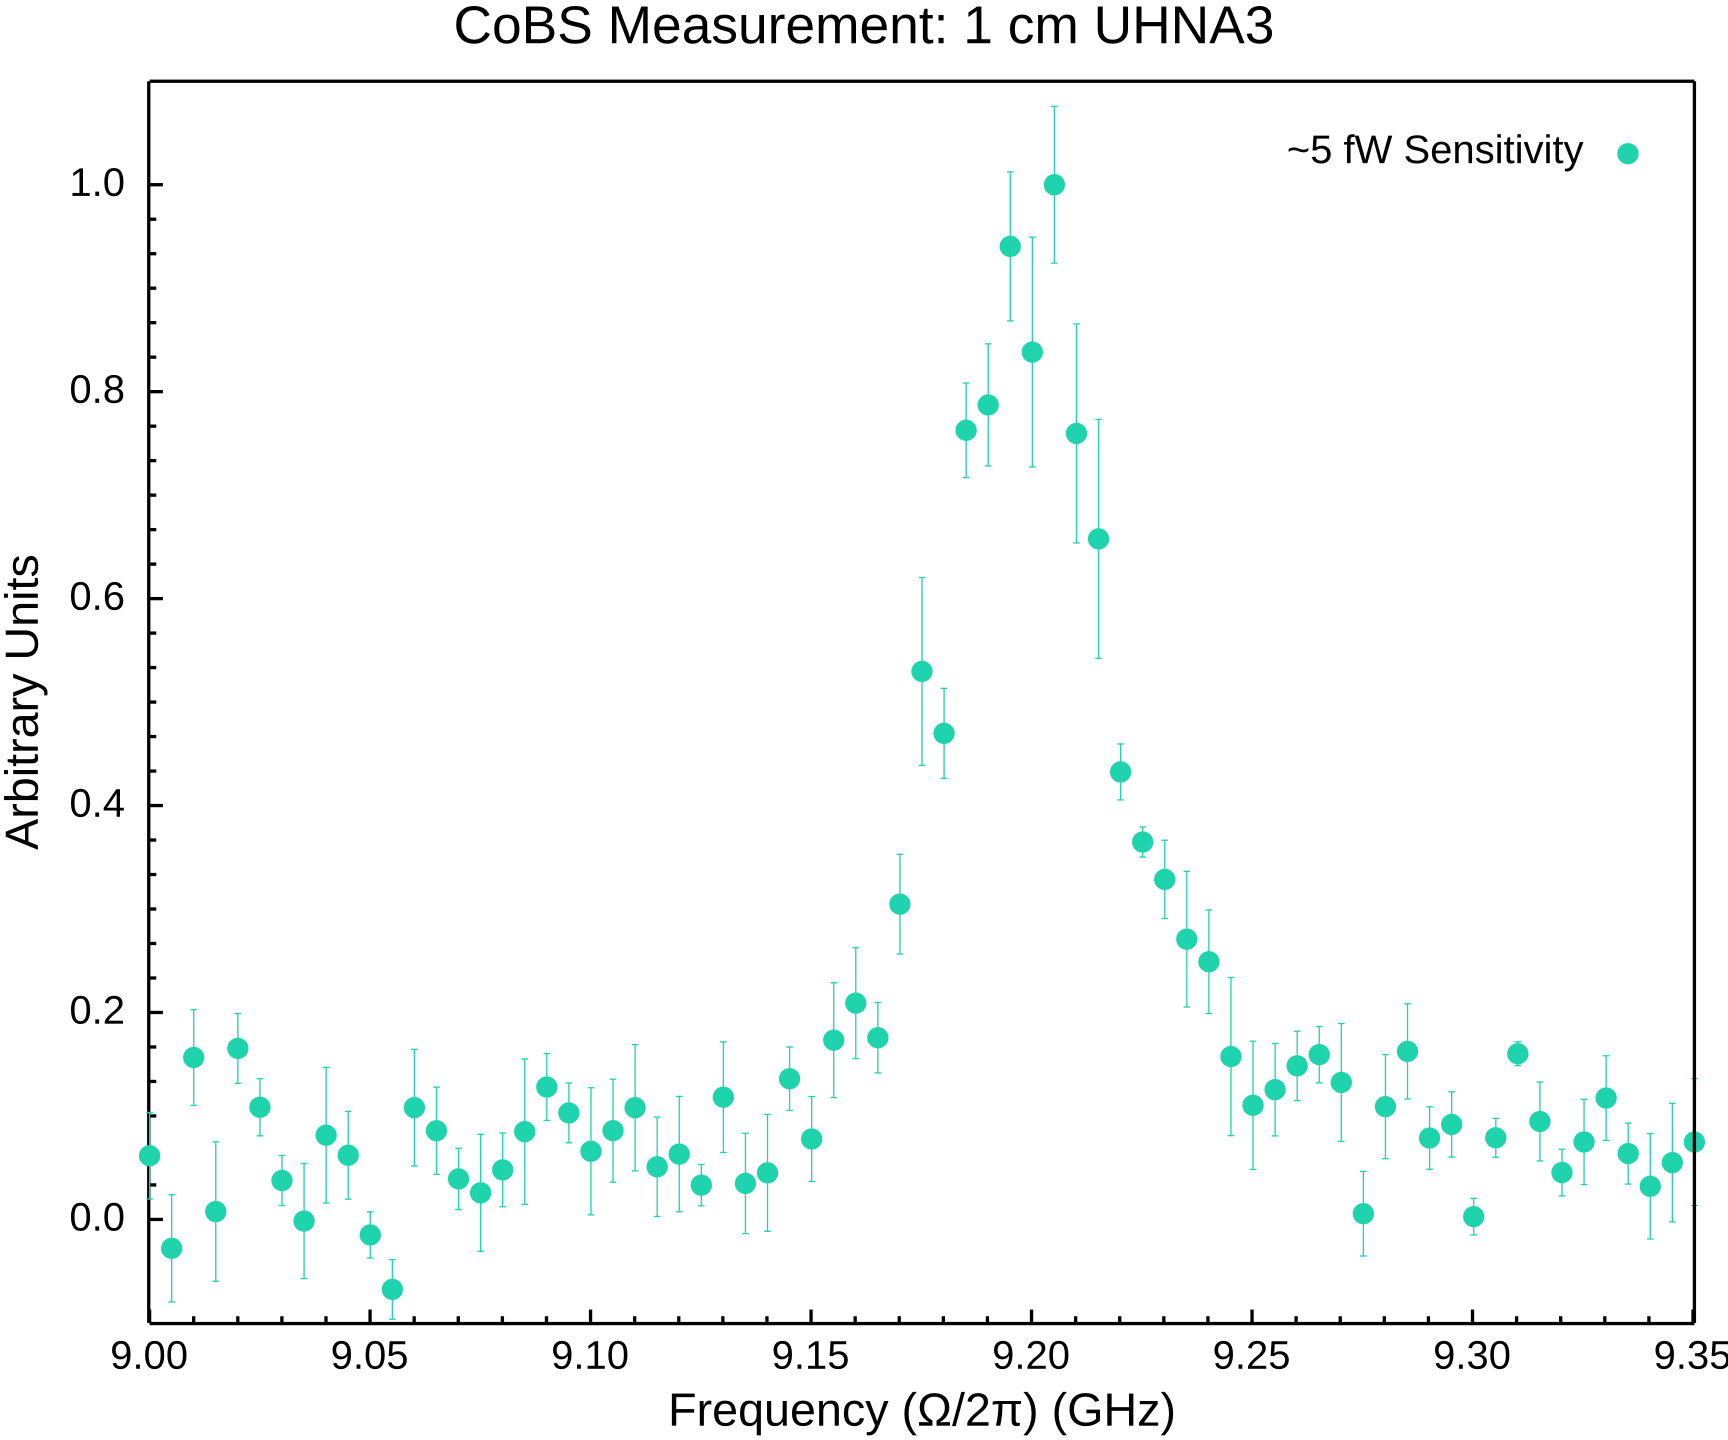
\includegraphics[width=.85\textwidth]{figs/3-CoBS/CoBS Sensitivity Measurement: 1 cm UHNA3 5 fW.png}
  \caption{Observed spectra demonstrating \(P_{\rm Signal}\approx\) \SI{5}{\femto\watt} sensitivity of the instrument. Experimental parameters for this measurement are tabulated in Table~\ref{tab:CoBS:5fWSensitivity}. In obtaining the spectra, five repeated measurements of both the signal and background (probe off) were collected at a \SI{100}{\hertz} \ac{RBW}, dwelling for \SI{1}{\second} at each \SI{5}{\mega\hertz} frequency step. Plotted is the resulting background-subtracted spectrum. Uncertainties represent 1\(\sigma\) standard error of the mean. By comparing the peak amplitude at resonance to the off-resonance baseline, we estimate an \ac{SNR} greater than 5, which, under a normal-noise assumption, corresponds to a \(5\sigma\) significance level (99.99994\% confidence).}
  \label{fig:CoBS:5fWSensitivity}
\end{figure}

Figure~\ref{fig:CoBS:5fWSensitivity} presents a measurement in which the instrument’s sensitivity reaches \(P_{Sig}\!= \SI{2}{\femto\watt}\). Table~\ref{tab:CoBS:5fWSensitivity} provides the experimental parameters used to gather this measurement and calculate the sensitivity. Each trace is the average of five consecutive scans, and an average of five background scans has been subtracted to isolate the signal. Error bars represent the standard error (\(1\sigma\) of the mean). By comparing the peak amplitude at resonance to the off-resonance baseline, we estimate an \ac{SNR} greater than 5. Under a normal-noise assumption, an \ac{SNR} of 5 corresponds to a \(5\sigma\) significance level (99.7\% confidence). Achieving this \SI{5}{\femto\watt} threshold demonstrates the feasibility of measuring weaker signals in materials with lower Brillouin gain or smaller effective lengths.

\begin{table}[h]
    \centering
    \begin{tabular}{c c c c c c c}
        \toprule
        \(\mathbf{G_{\mathrm{\textbf{B}}}}\) &
        \(\textbf{L}\) &
        \(\mathbf{P_{\mathrm{\textbf{P}}}}\) &
        \(\mathbf{P_{\mathrm{\textbf{S}}}}\) &
        \(\mathbf{P_{\mathrm{\textbf{Pr}}}}\) &
        \(\mathbf{\Delta\lambda}\) &
        \(\mathbf{\Phi}\) \\
        (\si{\per\watt\per\meter}) &
        (\si{\meter}) &
        (\si{\micro\watt}) &
        (\si{\micro\watt}) &
        (\si{\milli\watt}) &
        (\si{\pico\meter}) &
        \\
        \midrule
        0.6 & 0.01 & 506 & 504 & 2.01 & 20 & 0.90 \\
        \bottomrule
    \end{tabular}
    \caption{Experimental parameters used in observing \(P_{\rm Sig}\approx\) \SI{5}{\femto\watt} sensitivity of the \ac{CoBS} instrument. The resulting spectra is shown in Figure~\ref{fig:CoBS:5fWSensitivity}.}
    \label{tab:CoBS:5fWSensitivity}
\end{table}

\subsection{Measurements}
\label{Results:Measurements}

We demonstrate the capabilities of the instrument on two common sample classes: fiber and bulk material. For a fiber sample we again choose UHNA3 for its higher nonlinear response and excellent optical and acoustic guidance. In contrast to the sensitivity measurements, we now seek to demonstrate the full measuring capabilities of the instrument and so apply all available optical power (\(\sim\!\SI{1.5}{\watt}\)) to maximize the backscattered signal from the sample. We target the same \SI{1}{\centi\meter} segment of \ac{UHNA3} fiber as was used for determining sensitivity.

\begin{figure}[t!]
  \centering
  \hspace{-2em}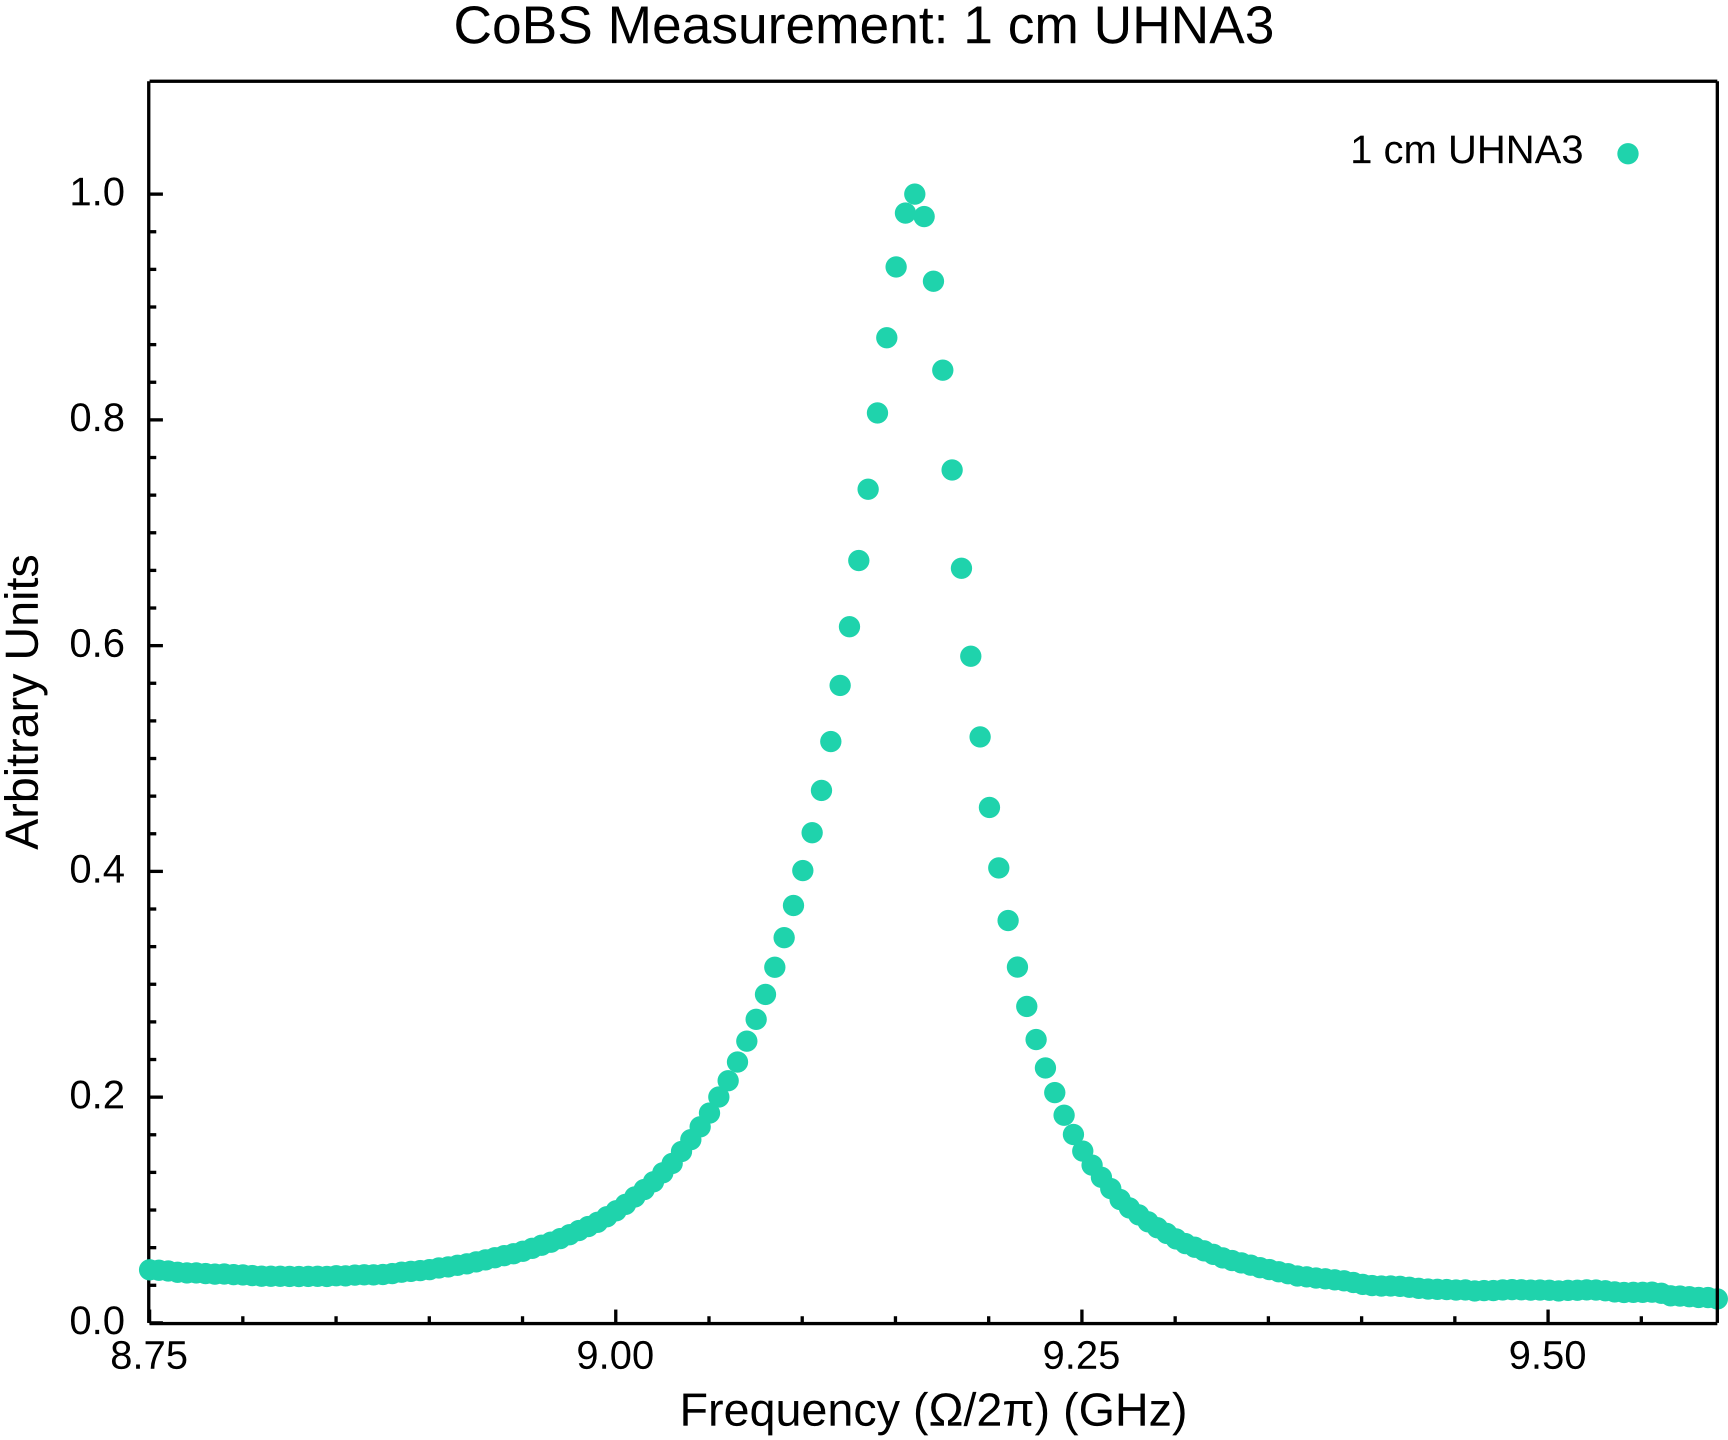
\includegraphics[width=.85\textwidth]{figs/3-CoBS/CoBS Measurement: 1 cm UHNA3.png}
  \caption{Observed spectra of \SI{1}{\centi\meter} \ac{UHNA3} fiber captured at maximum operating optical powers \(P_{\rm P}P_{\rm S}P_{\rm Pr} \sim\) \SI{0.25}{\cubic\watt}. The data exhibits the familiar Lorentzian profile for frequency-dependent dissipation probed by Brillouin scattering. This response is reflected in the \ac{CoBS} process gain \(G_{\rm CoBS}=\frac{1}{4}(G_{\rm B}L)^{2}P_{\rm P}P_{\rm S}P_{\rm Pr}\) given in Equation~\ref{Eq:Theoretical Framework:Scattered Power}, with Equation~\ref{Eq:Effective Brillouin Gain} for effective Brillouin gain offering the off-resonant Lorentzian lineshape. In obtaining the spectra, five repeated measurements of both the signal and background (probe off) were collected at a \SI{100}{\hertz} \ac{RBW}, dwelling for \SI{1}{\second} at each \SI{5}{\mega\hertz} frequency step. Plotted is the resulting background-subtracted spectrum, with 1\(\sigma\) uncertainties smaller than the data point markers.}
  \label{fig:1cmUHNA3}
\end{figure}

Figure~\ref{fig:1cmUHNA3} shows the spectral profile captured for \SI{1}{\centi\meter} of \ac{UHNA3} fiber, revealing the expected lorentzian profile consistent with Equation~\ref{Eq:Effective Brillouin Gain}. The peak amplitude of the spectra occurs at \SI{9.1704}{\giga\hertz}, indicating the Brillouin resonance frequency of the longitudinal traveling-wave mode in the fiber. The \ac{FWHM} linewidth of the measurement is \SI{80}{\mega\hertz} and provides a measure of the phonon dissipation rate. Both values match what is seen in the literature for \ac{SBS} measurements of \ac{UHNA3} fiber.\cite{behunin2015long} The data shown are a background-subtracted average of five successive measurements taken over ten minutes with error bars corresponding to \(1\sigma\) of the mean.

To achieve this measurement of \ac{UHNA3} fiber, the instrument design was altered to include only fiber-coupled segments connecting the fiber ports between the two \ac{PBS}s. We set the pump laser wavelength to \SI{1549.000}{\nano\meter} and the probe laser wavelength to \SI{1549.020}{\nano\meter}, giving a frequency mismatch of approximately \SI{2.5}{\giga\hertz}. The pump--probe mismatch is chosen to be only as large as needed to allow the edge of the pass-band of the probe filter to split the backscattered pump and probe light, thus rejecting any backscattered light from the pump laser and accepting only the backscattered signal from the probe laser. We placed the Stokes filter at \SI{1549.073}{\nano\meter}, an offet of approximately \SI{9.18}{\giga\hertz} from the pump laser to capture the Stokes sideband from the intensity modulator. This corresponds to the center of the measured frequency range and was chosen to allow the Stokes sideband output from the intensity modulator to remain within the pass band of the Stokes filter as the RF signal fed to the intensity modulator is swept through the full measurement range. The probe filter was set to \SI{1549.109}{\nano\meter}, an offset of approximately \SI{11.18}{\giga\hertz} from the probe laser, to capture the Stokes-shifted backscattered signal from the probe. The center frequency of the backscattered signal is of course shifted \SI{9.18}{\giga\hertz} from the probe laser, however an extra offset of \SI{2}{\giga\hertz} is chosen for improved rejection of any pump light as the pass band of our filter extends approximately \SI{2.5}{\giga\hertz} on either side of center.

\begin{figure}[t!]
  \centering
  \hspace{-2em}\includegraphics[width=.85\textwidth]{figs/3-CoBS/CoBS Measurement: 100 μm CS2.png}
  \caption{Observed spectra of \SI{100}{\micro\meter} liquid \ce{CS2} captured at maximum operating optical powers \(P_{\rm P}P_{\rm S}P_{\rm Pr} \sim\) \SI{0.25}{\cubic\watt}. Within the uncertainties, the data exhibits the familiar Lorentzian profile for frequency-dependent dissipation probed by Brillouin scattering. This response is reflected in the \ac{CoBS} process gain \(G_{\rm CoBS} = (G_{\rm B}L)^{2}P_{\rm P}P_{\rm S}P_{\rm Pr}\) given in Equation~\ref{Eq:Theoretical Framework:Scattered Power}, with Equation~\ref{Eq:Effective Brillouin Gain} for effective Brillouin gain offering the off-resonant Lorentzian lineshape. In obtaining the spectra, five repeated measurements of both the signal and background (probe off) were collected at a \SI{100}{\hertz} \ac{RBW}, dwelling for \SI{1}{\second} at each \SI{5}{\mega\hertz} frequency step. Plotted is the resulting background-subtracted spectrum. Uncertainties represent 1\(\sigma\) standard error of the mean.}
  \label{fig:100umCS2}
\end{figure}

For a free-space bulk example we target liquid \ce{CS2} for its exceptionally high Brillouin gain factor of \SI{1.5}{\meter\per\giga\watt}.\cite{boyd2020nonlinear} Figure~\ref{fig:100umCS2} reveals the Brillouin signal of bulk \ce{CS2} liquid contained in a \SI{100}{\micro\meter} path length cell. To our knowledge, measurement of longitudinal Brillouin scattering at this scale has not been reported in the literature. A scattered power comparison would reveal that achieving such a measurement using traditional \ac{SBS} techniques would require excessively high optical powers or cooling the material to cryogenic temperatures, which, of course, would be prohibitive for carbon disulfide in the liquid state.

For this measurement of \ce{CS2}, the pump and probe laser wavelengths were set to \SI{1548.808}{\nano\meter} and \SI{1548.898}{\nano\meter}, respectively. The short path length of the sample significantly broadens \(\Phi\), the \(\mathrm{sinc^2}\) term defining the phasematching bandwidth, allowing for further separation of the pump and probe wavelengths for improved signal isolation without significant reduction in scattered power of the signal produced in the \ce{CS2}. Specifically, the additional pump--probe wavelength separation of \SI{70}{\pico\meter} employed for this measurement compared to the UHNA3 measurement results in a negligible 0.045\% reduction in scattered power. This additional separation contributes meaningfully, however, to improved rejection of pump light by the probe filter and thus higher SNR of the signal.

Placement of the Stokes filter is critical for measurements of materials that give small Brillouin shifts, such as with \ce{CS2} \SI{2.55}{\giga\hertz} shift. We offset our \SI{5}{\giga\hertz} bandwidth Stokes filter an additional \SI{2}{\giga\hertz} to ensure the nearby carrier signal and anti-Stokes sideband from the intensity modulator are rejected and only the Stokes sideband is allowed to pass. For the measurement shown in Figure~\ref{fig:100umCS2}, this corresponds to a Stokes and probe filter placement of \SI{1548.844}{\nano\meter} and \SI{1548.934}{\nano\meter}, respectively.

% Figure~shows the spectral measurements achieved by the instrument, overlaid with finite-difference simulation data. In Figure~we see the expected lorentzian spectral shape in good alignment with simulation data for guided longitudinal modes in the core of the UHNA3 fiber. In Figure~, however, we see a distortion of this lorentzian shape. This is expected for partially unguided longitudinal modes, such as is the case for a bulk liquid filling the volume of a ...
%
% Figure~\ref{fig:1cmUHNA3} shows a measurement of 1cm of UHNA3 fiber.
%
% First, we measured Brillouin scattering in a 1-centimeter-long UHNA3 fiber at room temperature and with sub-Watt optical power (Figure~). Figure~, clearly displays the Brillouin scattering features with remarkable SNR, highlighting the effectiveness of our apparatus in isolating the backscattered probe light. This observation serves as one of the main showcases of the instrument's capability.
%
% Next, we performed Brillouin scattering measurements on a 4-millimeter-thick bulk carbon disulfide sample in a free-space optics arrangement. The observed spectrum, presented in Figure~2, exhibits well-resolved Brillouin scattering peaks. This successful measurement in a bulk sample demonstrates the versatility and adaptability of the instrument to various experimental configurations, further emphasizing the instrument's capability.
%
% Lastly, we conducted a measurement in a 1-millimeter-long UHNA3 fiber under low-power conditions, with only 10 microwatts of power at the sample. Despite the reduced sample length and low power, the instrument's sensitivity allowed us to observe distinct Brillouin scattering features in the spectrum, as illustrated in Figure~3. This result underscores the potential of our spectrometer for nanoscale measurements and serves as a demonstration of the instrument's sensitivity, defining the sensitivity floor of the apparatus.
%
% These three observations collectively showcase the high sensitivity, broad applicability, and impressive capabilities of our coherent stimulated phonon spectrometer in measuring Brillouin scattering across different sample types, scales, and power levels.

\subsection{Phase Matching Bandwidth}
\label{Results:Phase Matching Characterization}

To characterize the phase matching tolerance of the instrument for a given length of sample, we performed an additional experiment whereby we took a series of measurements of \SI{1}{\centi\meter} of UHNA3 at constant optical powers while letting the detuning of the pump and probe lasers vary. In the language of Equation~\ref{Eq:Theoretical Framework:Scattered Power}, this experiment holds \(G_B\), \(L\), \(P_P\), \(P_S\), and \(P_{Pr}\) constant while letting \(\Delta k\) vary. For the experiment to support the validation of Equation~\ref{Eq:Theoretical Framework:Scattered Power}, we would expect the peak amplitudes of these measurements to trace out a \(\mathrm{sinc^2}\) profile, also given by Equation~\ref{Eq:Phi}. Figure~\ref{fig:Phase-Match} shows the results of this experiment. We performed 75 measurements between \SI{5}{\giga\hertz} and \SI{42}{\giga\hertz} pump--probe detuning, at \SI{0.5}{\giga\hertz} intervals. We found peak amplitudes by fitting each spectra with a Fano profile (see Section~\ref{Results:Fano-Resonant Asymmetries at Small Signals}) and represented each peak as a data point in Figure~\ref{fig:Phase-Match}. The theoretical \(\mathrm{sinc^2}\) function matching the parameters used in the experiment is shown on the plot with a solid red line.

%Describe adjustments and/or explain deviations from pure sinc^2 (noise floor, Fano effects, L uncertainty, etc.), or reference Fano section

\begin{figure}[t!]
  \centering
  \hspace{-2em}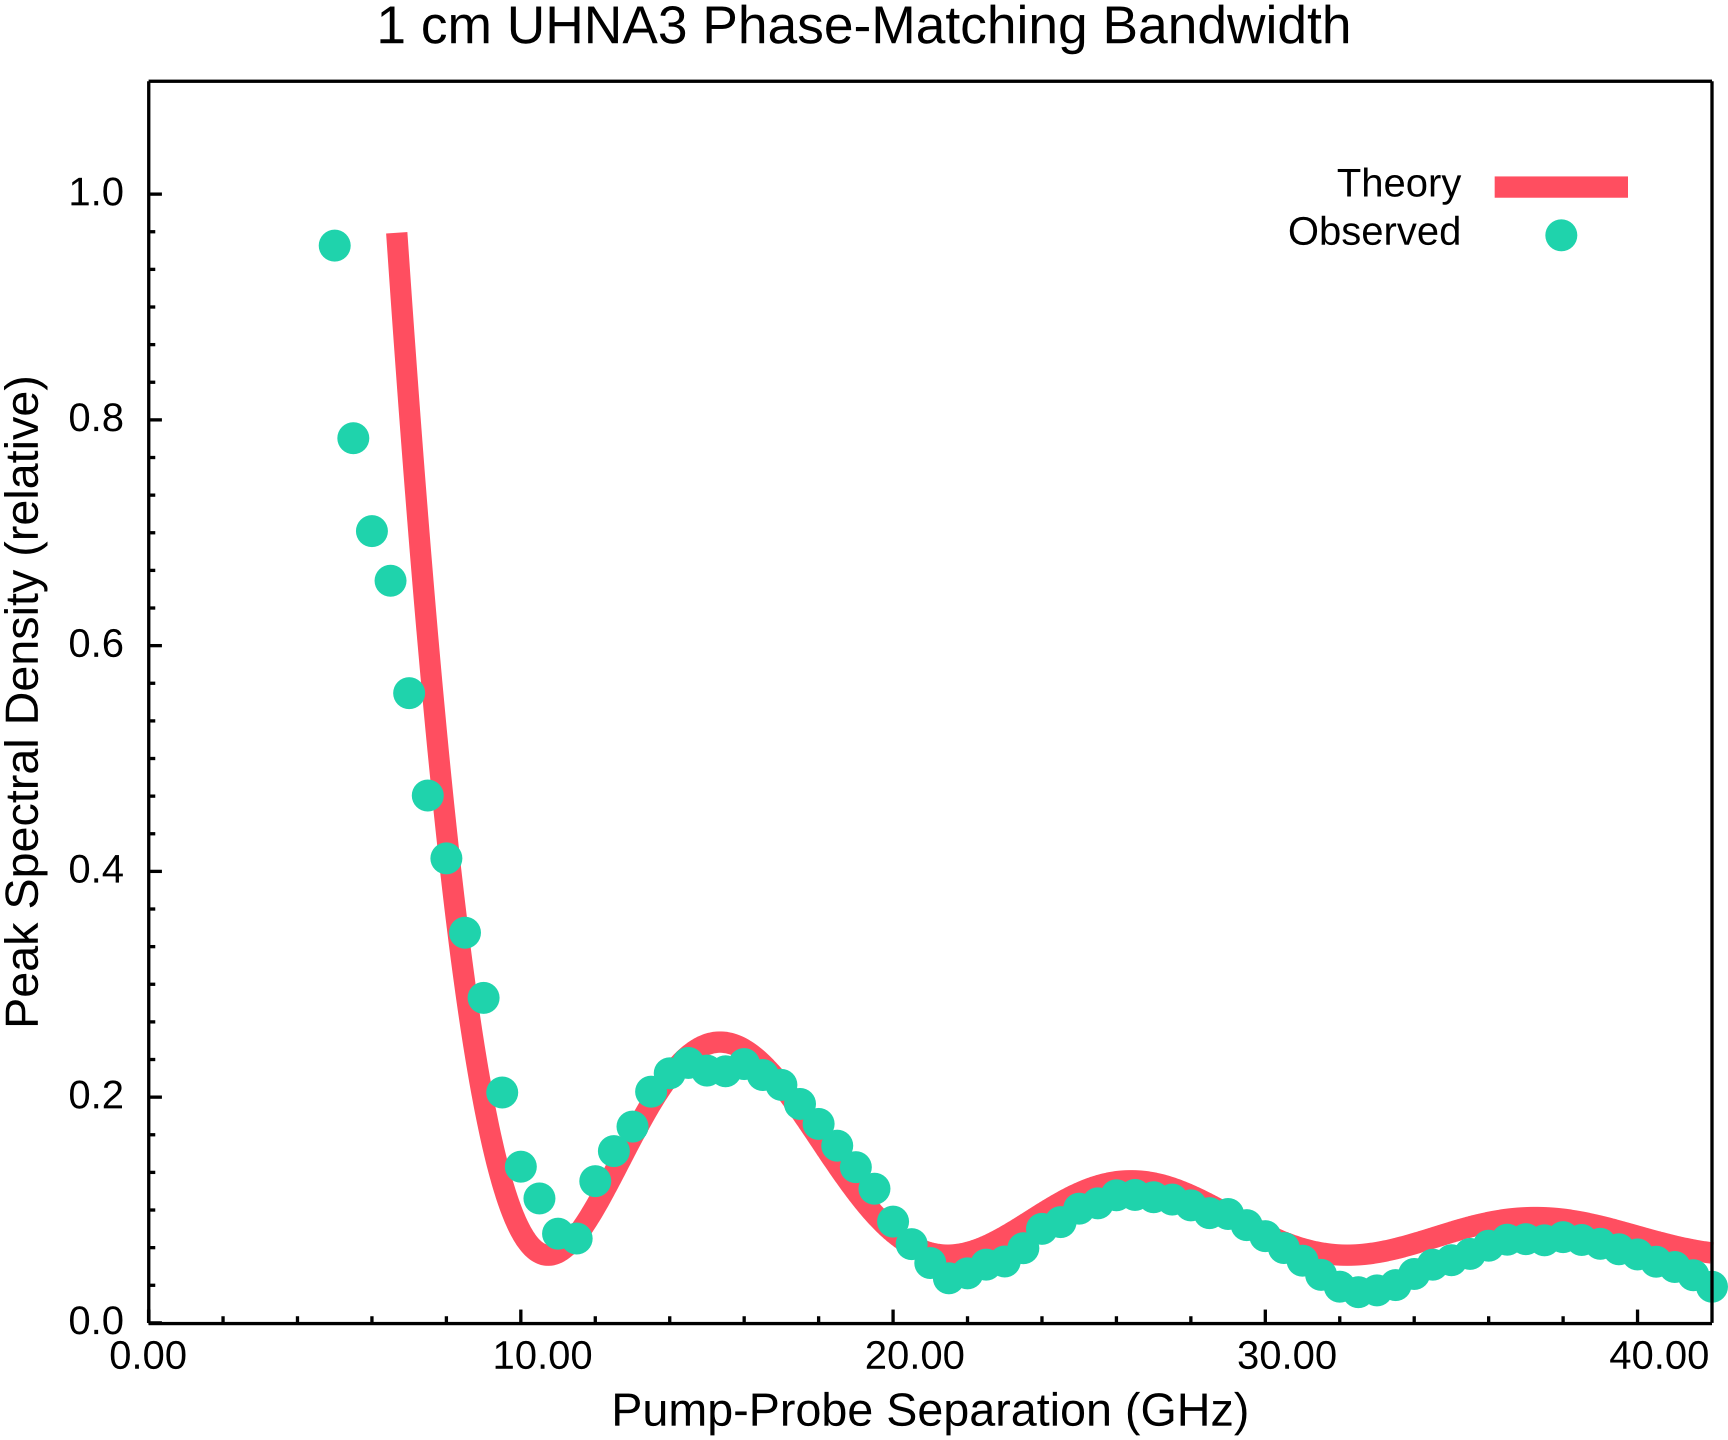
\includegraphics[width=.85\textwidth]{figs/3-CoBS/Phase-Match.png}
  \caption{Spectral peaks of 75 observed spectra of \SI{1(1)}{\centi\meter} \ac{UHNA3} across a range of pump-probe detunings (\(\omega_{\rm Pump} - \omega_{\rm Probe})/2\pi\)) from \SI{5}{\giga\hertz}-\SI{42}{\giga\hertz} in \SI{0.5}{\giga\hertz} increments. Values are obtained from uncertainty-weighted Fano fits of the observed spectra (see Appendix~\ref{Appendix:Fano}). The solid theoretical line shows the expected theoretical trend (a \(\mathrm{sinc^{2}}\) lineshape) given by Equation~\ref{Eq:Phi}, plotted here for the experimental parameters used in collecting the data and a fiber length of \(\sim\)\SI{0.9}{\centi\meter}. Section~\ref{Appendix:Fano:Experiment A} in Appendix~\ref{Appendix:Fano} offers an extended discussion of the observed spectra and contains a plot of the full set of 75 spectra (Figure~\ref{Appendix:Fano:Experiment A}). In obtaining each spectra, five repeated measurements of both the signal and background (probe off) were collected at a \SI{100}{\hertz} \ac{RBW}, dwelling for \SI{1}{\second} at each \SI{5}{\mega\hertz} frequency step. Uncertainty-weighted Fano fits were computed from the resulting background-subtracted spectra. Plotted here are the fit-extracted spectral peaks, with 1\(\sigma\) uncertainties smaller than the data point markers.}
  \label{fig:Phase-Match}
\end{figure}

\subsection{Fano-Resonant Asymmetries at Small Signals}
\label{Results:Fano-Resonant Asymmetries at Small Signals}

Under certain conditions where the resonant Brillouin amplitude approaches the background continuum level, we observe an asymmetric, Fano‐type line-shape \cite{fano1961effects, limonov2017fano, limonov2021fano, kroner2008nonlinear}. These Fano distortions can shift the apparent peak frequency, complicate simple Lorentzian fitting, and affect the extracted linewidth in small‐signal measurements. \cite{miroshnichenko2010fano} To properly handle these occurances, it is necessary to understand when they are likely to arise with this technique and how they may be corrected for or controlled. Fano resonances arise when a discrete resonance (in our case, the Brillouin mode) interferes with a continuum background (e.g., noise floor or broad, non‐resonant scattering). When the resonance amplitude is no longer much larger than the continuum, the interference leads to an asymmetric line-shape described by the Fano formula \cite{fano1961effects},

\begin{equation}
I(\omega) \propto \frac{(q + \epsilon)^2}{1 + \epsilon^2},
\label{eq:fano}
\end{equation}

where \(\epsilon \equiv (\Omega - \Omega_{B})/(\Gamma_{B}/2)\) is the dimensionless detuning from the Brillouin peak (measured in half the spectral linewidth) and \(q\) is the Fano asymmetry parameter. The Fano asymmetry parameter captures the ratio of the resonant scattering to the background scattering amplitudes as well as the relative phase of each. It can be defined as

\begin{equation}
  q = \frac{(\mathrm{resonant amplitude})}{(\mathrm{background amplitude})}\cot{(\Delta\phi)},
\end{equation}

where \(\Delta\phi\) is the phase difference between the oscillation driven by the discrete resonant mode and that of the background continuum \cite{limonov2017fano, ko2023full, gu2020fano}.

In the event of Fano interference, the complex background amplitude often varies slowly with energy and can be seen as having a fixed phase reference, while the resonant amplitude undergoes a rapid \(\pi\) phase change as the energy passes through the resonance. \cite{limonov2017fano} When the resonant and background contributions are exactly out of phase at the resonance frequency (phase difference \(\Delta\phi = \pi/2\), meaning destructive interference), the spectral line exhibits a dib to zero (anti-resonance) at the discrete resonance frequency, corresponding to \(q=0\) in Equation~\ref{eq:fano}. If they are exactly in phase (\(\Delta\phi = 0 or \pi\), fully constructive interference at resonance), the resonance appears purely Lorentzian without asymmetry and \(|q| \to \infty\). For intermediate phase offsets, one lobe of the resonance is enhanced while the other is suppressed, yielding an asymmetric peak or dip with finite \(q\). The sign of q indicates the direction of asymmetry (which wing of the resonance is enhanced). A positive \(q\) means the discrete mode \textit{leads} the background in phase. In this case, the spectral profile has a sharp rise on the low-frequency side and a more gradual fall-off on the high-frequency side. Conversely, a negative \(q\) means the discrete mode \textit{lags} the background in phase, leading to a flipped orientation featuring a sharp rise on the \textit{high}-frequency side and a gradual fall-off on the \textit{low}-frequency side.

We first noticed this behavior appearing in our small-length \ce{CS2} data, where a small shift in probe wavelength revealed an asymmetric line-shape. For the measurements of \SI{100}{\micro\meter} \ce{CS2} (Figure~\ref{fig:100umCS2}) and \SI{1}{\centi\meter} \ac{UHNA3} fiber at low power (Figure~\ref{fig:CoBS:5fWSensitivity}), the amplitude of the resonant Brillouin peak is on the order of that of the non‐resonant continuum, giving a strong chance for Fano interference. Whenever \(\tfrac{I_{\text{res}}}{I_{\text{bkg}}}\approx 1\), the parameter \(q\) as given by Equation~\ref{eq:fano} can become finite rather than \(\pm \infty\) in the limit that the background is negligible, and Fano interference arises. To explore this further, we performed a similar phase-matching experiment as was done for \SI{1}{\centi\meter} \ac{UHNA3} (see Phase Matching Bandwidth subsection), this time with \SI{1}{\milli\meter} of \ce{CS2}. Results from this experiment are presented in Appendix~\ref{Appendix:Fano} and offer examples of line shapes with pronounced asymmetry and featuring clear characteristic morphologies associated with Fano interference. These pronounced distortions in spectral line shape for small signal measurements underscore the role Fano interference in small resonant amplitudes relative to the background.

Because our instrument offers sub-\SI{10}{\femto\watt} sensitivity signal amplitudes have the potential to approach the order of the background continuum amplitude. For this reason, and because the instrument offers an advantage in measurements of samples of short length (\(<\)\SI{10}{m}) (see Appendix~\ref{appendix:comparison}), Fano effects may often arise with usage of this technique and must be handled appropriately. This includes properly fitting data with a Fano profile as opposed to a Lorentzian to ensure accurate capture of relevant parameters such as linewidth, resonant frequency, and peak amplitude. Beyond fitting and parameter extraction, it is important to be mindful that these effects are likely to occur in ambitious measurements at the limits of equipment sensitivity. Expectation and proper handling of Fano effects in measurements of this nature ensures that they may be more easily recognized and confirmed, as the data is likely to present a spectrum that deviates considerably from the standard Lorentzian. Appendix~\ref{appendix:comparison} offers a comparative analysis of two example spectra featuring highly assymetric profiles fitted with a naïve Lorentzian vs. a more appropriate Fano function.

In some cases, and of particular interest for ambitious measurements, Fano interference may even \textit{boost} the measured peak above the naïve Lorentzian amplitude—i.e., ‘amplify’ it—when \(q \neq 0\). In principle, a Fano‐type lineshape can exhibit a locally higher peak amplitude than a pure Lorentzian if the discrete Brillouin response constructively interferes with the background continuum near the resonance. Crucially, this does not represent net energy gain but rather a redistribution of intensity through interference. Although the resonance peak may appear taller, the continuum also contributes noise and can partially interfere destructively elsewhere, so the global \ac{SNR} may or may not improve. Nonetheless, our technique offers the ability to dynamically tune the phase of the Brillouin response relative to the background via adjustment of the probe laser wavelength. This interference-tuning of the continuum and discrete components allows some control over constructive or destructive interference. Moreover, we can achieve this without sacrificing independent control of the pump–probe detuning: by simultaneously shifting the pump laser in step with the probe, we can preserve the desired phase‐matching bandwidth while optimizing the relative phase for Fano interference.

In the phase‐matching bandwidth experiment on \SI{1}{\centi\meter} of \ac{UHNA3} fiber (Figure~\ref{fig:Phase-Match}), several effects—noise floor, alignment drifts, fiber dispersion, etc.—slightly distort the ideal \(\mathrm{sinc^{2}}\) response. Near the troughs of the \(\mathrm{sinc^{2}}\) function and for larger pump–probe detunings, the measured Brillouin peaks are weaker and exhibit small spectral asymmetries (see Appendix~\ref{Appendix:Fano}). This is consistent with a Fano‐type distortion in which the Brillouin amplitude and background continuum are comparable, allowing interference to skew the lineshape and shift the peak away from the naïve Lorentzian center. Consequently, a simple Lorentzian fit underestimates the true peak amplitude in these regimes. By fitting a standard Fano profile, we more accurately capture the asymmetric peak and its shifted center frequency.

\section{Conclusion}
\label{Conclusion}

In conclusion, we have introduced a coherently stimulated Brillouin spectrometer utilizing a detuned pump-probe design to achieve high sensitivity and room-temperature operation in \si{\micro\meter}-scale samples. This approach successfully overcomes the spatial resolution limitations imposed by conventional \ac{SBS} methods, demonstrating sub-\SI{10}{\femto\watt} sensitivity in \ac{UHNA3} fiber and enabling Brillouin measurements in bulk liquid carbon disulfide with unprecedented efficiency. By relaxing phase-matching constraints, this instrument opens new possibilities for characterizing nanoscale material properties and developing nano-acousto-optic devices in standard laboratory settings without the need for cryogenic environments. Moving forward, our methodology could facilitate advancements in high-resolution phonon spectroscopy and inspire further innovations in the study of material mechanics at the microscale, reinforcing the broader applicability of Brillouin-based techniques across materials science, photonics, and sensing technologies.

\clearpage
\thispagestyle{empty}
\null
\newpage
